% !TEX root = _individual/trtBackground.tex

%%%%%%%%%%%%%%%%%%%%%%%%%%%%%%%%%%%%%%%%%%%%%%%%%%%%%%%%%%%%%%%%%%%%%%%%%%%%%%%%
\chapter{Background to Thermal Radiative Transfer}\label{chap:trtBackground}

To elucidate the derivation of the anisotropic
diffusion approximation, it is necessary to delve into the physical
process of radiation transport. As discussed in the introduction,
thermal radiative transfer is the physical process of energy transfer via
high-energy photons in hot materials. Because the TRT equations and
approximations have been probed and reviewed in other works
\cite{Mih1984,Pom1973,Cas2004,Wol2008}, our aim is a concise explanation of the
physics relevant to the anisotropic diffusion approximation and its immediate
application, rather than a thorough overview of the extensive field of radiation
hydrodynamics. We also review the derivation of competing solution methods and
discuss their advantages and shortcomings.

%%%%%%%%%%%%%%%%%%%%%%%%%%%%%%%%%%%%%%%%%%%%%%%%%%%%%%%%%%%%%%%%%%%%%%%%%%%%%%%%
\section{Nonlinear radiation transport}\label{sec:bgTrtEquations}
Thermal radiative transfer describes the motion of high-energy photons
in a very hot material, such as the interior of a star or the target of a laser
fusion experiment. The equations that model TRT are time-dependent, contain
strong nonlinearities, and reside in a large phase space.
A full representation of the physics in
the high-energy-density regime often includes the consideration of moving
relativistic materials, different electron and ion temperatures, photon
scattering, and thermal conduction in the material \cite{Mih1984}. However,
much work in the methods development field neglects these complex phenomena by
\begin{itemize}
  \item working in a fixed medium, disregarding material advection;
  \item assuming local thermodynamic equilibrium (LTE), which uses a single
    material temperature;
  \item neglecting photon scattering, which tends to be small;
  \item neglecting thermal conduction, since energy transfer is dominated by
    radiation at high temperatures;
  \item applying the ``gray'' (monoenergetic) approximation to the frequency
    dependence by integrating the full transport equation over all $\nu$, averaging 
    the
    opacities with a suitable \emph{a priori} weighting function \cite{Lar1983a}.
\end{itemize}

For the purposes of discussion and the later AD derivation, we consider a
general, 3-D universe, in which the spatial coordinates $x$, $y$, and $z$ define a
spatial point
\begin{equation*}
  \vec{x}
  = x \vec{i} + y \vec{j} + z \vec{k}\,,
\end{equation*}
and the angular coordinates $\mu$ and $\theta$ define an arbitrary unit
vector denoting the direction of flight:
\begin{equation*}
  \vec{\Omega}
  = \mu \vec{i}
  + \sqrt{1-\mu^2} \cos \theta \vec{j}
  + \sqrt{1-\mu^2} \sin \theta \vec{k} \,.
\end{equation*}
These angular coordinates reside in the domain $-1 \le \mu \le 1$, $0 \le \theta
< \pi$; we use $\vec{\Omega}\in4\pi$ as a shorthand denoting the entire
unit sphere. See \cite{Lar2007,Pri2010} for a more complete discussion of the
spatial and angular coordinate systems.

\subsection{Equations of transfer}
After the simplifications described above, the thermal radiative transfer
process in the interior of a problem (away from the initial time and
from boundaries) can be described \cite{Pom1973} by
\begin{subequations} \label{eqs:explanTRT}
the gray radiative transfer equation,
\begin{equation} \label{eq:explanTransport}
  \frac{1}{c} \pder{I}{t}
  + \vec{\Omega} \vd \del I +
 \sigma I
  = \frac{\sigma a c T^4}{4\pi} 
  + \frac{q_r}{4\pi} \,,
\end{equation}
and the material energy balance equation,
\begin{equation} \label{eq:explanMaterial}
  c_v \pder{T}{t} = \sigma \int_{4\pi}  I \ud \Omega - \sigma a c T^4
  + q_m \,.
\end{equation}
\end{subequations}

The notation and omitted parameters in Eqs.~\eqref{eqs:explanTRT} are:
\begin{alignat*}{2}
  I &= I(\vec{x}, \vec{\Omega}, t) &&= \text{the angular
  radiation intensity,}
  \\
  T &= T(\vec{x}, t) &&= \text{the material temperature,}
  \\
  \sigma &= \sigma(\vec{x}, T) &&= \text{the absorption opacity,} 
  \\
  q_r &= q_r(\vec{x}, t) &&= \text{an extraneous isotropic radiation energy source,}
  \\
  q_m &= q_m(\vec{x}, t) &&= \text{an energy source in the material,}
  \\
  c_v &= c_v(\vec{x}, T) &&= \text{the specific heat capacity of the material,}
  \\
  a& &&= \text{the radiation constant, and}
  \\
  c& &&= \text{the speed of light.}
\end{alignat*}
The intensity $I$ and the temperature $T$ are the primary unknowns: they
describe the state of energy in the radiation and in the material.
Each of the terms that depends on $T$ implicitly depends on the time $t$. The
explicit dependence of $c_v$ and $\sigma$ on $\vec{x}$ accounts for different
materials in different parts of the problem.

Equation~\eqref{eq:explanTransport} is a transport equation for $I$. The first
two terms describe how photons ``stream'' in time and space: if the
other terms were zero, Eq.~\eqref{eq:explanTransport} would reduce to a
wave equation with a wave speed of $c$. However, because the photons move 
through a material, there is a chance they will collide with its electrons,
hence the \emph{collision} term $\sigma I$. The first term on the right-hand
side represents particles emitted via the isotropic temperature-dependent
process of \emph{black body emission}. The additional term $q_r$ is an extraneous
isotropic radiation source that emits with an energy density (energy per
volume per time) of $q_r$.

The material equation~\eqref{eq:explanMaterial} describes an energy balance in
the material. The left-hand side is the time rate of change in the material
energy density. The first term on the right-hand side exactly mirrors the collision term in the
radiation equation: it is a ``gain'' term corresponding to photons that
collided with (were absorbed by) the material. The second term describes the loss
of energy from the material when it emits black body radiation. The material
energy source, or electron source, is sometimes used in numerical test problems
\cite{Ada2010}.

The physical properties $\sigma$ and $c_v$ are often approximated by simplistic
models in the methods development literature. The heat capacity $c_v$ of an ideal
gas is a constant, giving the material energy a linear proportionality to
the material temperature $T$. A much-used model \cite{Mou2006,Wol2008} of the
gray opacity is $\sigma \propto T^{-3}$.
Our numerical test problems will use both of these idealized representations of
the physical constants.

The nonlinear coupling between Eqs.~\eqref{eq:explanTransport}
and~\eqref{eq:explanMaterial} via $T^4$ emission and $T^{-3}$ absorption make
the TRT equations extremely ``stiff'' \cite{Kno2003} and therefore even more
difficult to solve than the standard linear transport equation. In this work,
we will not attempt to provide any new solutions to treat the nonlinearities,
but we will formulate our time-dependent anisotropic diffusion approximations to
be compatible with multiple solution techniques.

\subsection{The radiation intensity}

The state of the photons in a system is described by the radiation
\emph{photon density},
\begin{align*}
  N(\vec{x},\vec{\Omega}, \nu, t) \ud V \ud \Omega
  &= \topbox{the number of photons inside the differential volume $\ud V$
  about $\vec{x}$, traveling in the directions $\Omega$ about
  $\vec{\Omega}$, inside the frequencies $\ud \nu$ about $\nu$, at time $t$.}
\end{align*}
However, because the photon energy $h\nu$ determines the energy
density of the radiation, and because the reaction rate with the material
depends on the photons' speed $c$, the radiation field is almost always written
as the \emph{radiative intensity},
\begin{equation*}
  I(\vec{x},\vec{\Omega},\nu, t) = c h\nu N(\vec{x},\vec{\Omega},\nu, t)\,.
\end{equation*}
The frequency-dependent intensity $I$ is an energy-weighted radiation path
length density, similar to the angular flux $\psi$ in reactor physics.%
\footnote{Note that $\psi$ is not weighted by energy, because neutrons' energy
primarily determines their interaction cross section; photons in contrast are
the means of energy transfer in the regimes considered in this thesis.}

Integrating over all energy gives the gray intensity, which we use from this point forward:
\begin{equation*}
  I(\vec{x},\vec{\Omega}, t)
  = c \int_0^\infty h\nu N(\vec{x},\vec{\Omega},\nu, t) \ud\nu \,.
\end{equation*}

Additionally, integrating over all angles (i.e.~taking the zeroth angular
moment) yields the \emph{scalar intensity}
\begin{align} \label{eq:intensityZeroth}
  \phi(\vec{x},t) &\equiv \int_{4\pi} I(\vec{x},\vec{\Omega}, t) \ud \Omega
  \\
  &= c \int_{4\pi} \int_0^\infty h\nu N(\vec{x},\vec{\Omega},\nu, t) \ud\nu
   \ud \Omega
\\ \intertext{which is directly proportional to the \emph{radiation energy
density}:}
\nonumber
\frac{1}{c} \phi(\vec{x},t) \ud V
&= \topbox{the amount of energy in the radiation field inside the differential
  volume $\ud V$ about $\vec{x}$, at time $t$.}
\end{align}
For our work, it is usually more convenient to refer to $\phi$ than to the
radiation energy density (compare, for example, \cite{Den2007} to
\cite{Kno1999a}). In fact, since our computational experiments use the
scaled system of variables $c=a=1$, our later results can use ``scalar
intensity'' and ``radiation energy density'' interchangeably.

The first angular moment of the intensity also has physical significance. The
\emph{radiation flux} is defined as
\begin{equation} \label{eq:intensityFirst}
  \vec{F}(\vec{x},t) \equiv \int_{4\pi} \vec{\Omega}
  I(\vec{x},\vec{\Omega}, t) \ud \Omega \,.
\end{equation}
Analogous to the ``neutron current'' $\vec{J}$ in reactor physics, the
radiation flux is the net rate and direction of energy flowing through a point.

At any particular point in space and time, the radiation intensity $I$ is
generally a complicated function of angle.
%\footnote{See \cite{Ada2001a} for an example of how complicated a function of
%angle the transport solution can be in even a simple reactor physics problem.}
For example, at the edge of a
radiation shock wave, the distribution is highly peaked in the directions
pointed away from the hot region, because that is the source of the photons. In
parts of the problem where the system is closer to an equilibrium state,
the intensity is nearly isotropic (almost uniform in angle).

%%%%%%%%%%%%%%%%%%%%%%%%%%%%%%%%%%%%%%%%%%%%%%%%%%%%%%%%%%%%%%%%%%%%%%%%%%%%%%%%
\section{Semi-implicit linearization}\label{sec:bgSemiImplicit}

The anisotropic diffusion approximation is best implemented as a deterministic
method. It is
therefore necessary to discuss \emph{discretization} schemes,
in which the continuous unknowns in Eqs.~\eqref{eqs:explanTRT} are approximated
with discrete unknowns. In this section, we discuss the discretization of the
time variable in the context of \emph{linearization}, which approximates
the nonlinear aspects of the TRT equations to allow a linear algebraic
representation of the system of unknowns, facilitating their solution on a
computer.

The common
``semi-implicit'' scheme uses operator splitting
to decouple the radiation and material equations inside a time step; the
remaining time-dependent unknowns are treated with the backward Euler
discretization \cite{Kno1999a,Kno2001,Low2004}.
Like Fleck and Cummings' IMC method \cite{Fle1971}, this technique
yields a linear transport equation with a pseudo-scattering term. Because of the
extensive use of this
nonlinear treatment in our implementations of anisotropic diffusion and the
other tested methods, and because the semi-implicit scheme for radiation
transport is usually glossed over in other works, we derive
it here in a practical level of detail. Existing derivations also omit the
\emph{material source} term $q_m$.

For the semi-implicit discretization, it is convenient to write
Eqs.~\eqref{eqs:explanTRT} in a slightly altered form:
\begin{subequations} \label{eqs:semiTRT}
\begin{equation} \label{eq:semiTransport}
  \frac{1}{c} \pder{I}{t}
  + \vec{\Omega} \vd \del I +
 \sigma I
 = \frac{\sigma c U_r}{4\pi} 
  + \frac{c q_r}{4\pi} \,,
\end{equation}
and the material energy balance equation,
\begin{equation} \label{eq:semiMaterial}
  \pder{U_m}{t} = \sigma \phi - \sigma c U_r + q_m \,.
\end{equation}
\end{subequations}
Here, we have defined the \emph{material energy density}, which is a function of
the
material's temperature and specific heat capacity $c_v$:
\begin{equation} \label{eq:matEnergyDens}
  U_m(T) = \int_{0}^{T} c_v(T') \ud T' \,,
\end{equation}
and the \emph{equilibrium radiation energy density} of a
material, which is a scaled integral of the Planckian emission function:
\begin{equation} \label{eq:radEnergyDens}
  U_r(T) \equiv aT^4
  = \frac{1}{c} \int_{4\pi} \int_{0}^{\infty} B(\nu, T) \ud\nu \ud\Omega \,.
\end{equation}
Its physical relevance is that, when the radiation field and material reach
an equilibrium, the radiation intensity becomes the Planck function $I=B$, and
the radiation energy density $\phi/c$ is equal to
$U_r$.  The quantity $U_r$ is \emph{not} equal to the energy density stored in
the material, $U_m$.

Note here that Eqs.~\eqref{eqs:semiTRT} are two equations with three unknowns:
$I$, $U_r$, and $U_m$. However, $U_r$ and $U_m$ are both properties of the
material---%
explicit functions of the material temperature $T$---%
so there are only two
underlying unknowns: one describing the radiation state (intensity), and the
other describing the material state (temperature).

\subsection{Linearizing the material energy equation}

To proceed, we define a parameter $\beta$ as a function of
Eqs.~\eqref{eq:matEnergyDens} and~\eqref{eq:radEnergyDens}:
\begin{equation} \label{eq:beta}
  \beta(\vec{x}, T) \equiv \pder{U_r}{U_m} 
  = \pder{U_r}{T} \Bigg/ \pder{U_m}{T}
  = \frac{4 a T^3}{c_v(\vec{x}, T)} \,.
\end{equation}
The chain rule allows the left hand side of Eq.~\eqref{eq:semiMaterial} to be
expressed without approximation in terms of the equilibrium radiation energy
density $U_r$:
\begin{equation*}
  \pder{U_m}{t} = \pder{U_m}{U_r} \pder{U_r}{t} = \frac{1}{\beta(T)}
  \pder{U_r}{t} = \sigma \phi - \sigma c U_r + q_m \,.
\end{equation*}
The first approximation is to ``freeze'' the parameter $\beta$ at the
beginning-of-time-step temperature $T^n$:
\begin{equation*}
  \beta[\vec{x},T(\vec{x},t)] \approx \beta[\vec{x},T(\vec{x},t^n)]
  = \beta(\vec{x}, T^n) \equiv \beta^n(\vec{x})\,,
\end{equation*}
so Eq.~\eqref{eq:semiMaterial} becomes for $t^n < t < t^{n+1}$
\begin{equation}\label{eq:frozenBeta}
  \frac{1}{\beta^n}
  \pder{U_r}{t} \approx \sigma \phi - \sigma c U_r \,.
\end{equation}
The process of freezing $\beta$ is equivalent to approximating the
material energy term using two first-order Taylor series:
\begin{align} \nonumber
  U_m(t^{n+1})
  &\approx U_m(t^n) + (t^{n+1} - t^n) \pder{U_m}{t}\bigg|_{t^n} + O( (t^{n+1} - t^n)^2)
  \\ \nonumber
  U_m^{n+1}
  &= U_m^n + \Delta_t \pder{U_m}{U_r}\bigg|_{t^n} \pder{U_r}{t}\bigg|_{t^n}
  + O( \Delta_t^2 )
  \\ \nonumber
   U_m^{n+1}
   &= U_m^n + \Delta_t \frac{1}{\beta^n} \left[ \frac{U_r^{n+1} - U_r^n}{\Delta_t} +
  O(\Delta_t) \right]
  + O( \Delta_t^2 )
  \\ \nonumber
   U_m^{n+1}
  &= U_m^n + \frac{U_r^{n+1} - U_r^n}{\beta^n} + O( \Delta_t^2 )
  \\
  \label{eq:matenConservationUpdate}
  U_m^{n+1}
  &\approx U_m^n + \frac{U_r^{n+1} - U_r^n}{\beta^n} \,.
\end{align}
Because the freezing of $\beta$ approximates the rate of change
in material energy, Eq.~\eqref{eq:frozenBeta} no longer conserves the system's
total energy. To enforce conservation of energy over a time step, we use
Eq.~\eqref{eq:matenConservationUpdate}.

The next approximation explicitly freezes the opacity $\sigma$ in
Eq.~\eqref{eq:frozenBeta}:
\begin{equation*}
  \frac{1}{\beta^n}
  \pder{U_r}{t} \approx \sigma^n \phi - \sigma^n c U_r + q_m \,.
\end{equation*}
Now we can average the material equation in time to express it in terms of two
simple unknowns. Operating by
$\frac{1}{\Delta_t^n}\int_{t_n}^{t^{n+1}} (\cdot) \ud t$,
we obtain
\begin{equation*}
  \frac{1}{\beta^n}
  \frac{U_r^{n+1} - U_r^n}{\Delta_t^n} = \sigma^n \left[
  \frac{1}{\Delta_t^n}\int_{t_n}^{t^{n+1}} \phi \ud t
  \right] - \sigma^n c \left[
  \frac{1}{\Delta_t^n}\int_{t_n}^{t^{n+1}} U_r \ud t \right]
   + \frac{1}{4\pi}\left[
  \frac{1}{\Delta_t^n}\int_{t_n}^{t^{n+1}} q_m \ud t \right]\,.
\end{equation*}
Next, we apply the implicit Euler discretization%
\footnote{Note that the IMC method only applies the implicit approximation to
$U_r$, allowing the continuous-in-time treatment of the intensity.}
to $U_r(\vec{x}, \vec{\Omega}, t)$ and $\phi(\vec{x}, \vec{\Omega}, t)$ by
approximating their time-averaged values as their values at the end of the time
step $t^{n+1}$:
\begin{equation} \label{eq:semiImplicitMaterial}
  \frac{1}{\beta^n(\vec{x})}
  \frac{U_r^{n+1}(\vec{x}) - U_r^n(\vec{x})}{\Delta_t^n}
  = \sigma^n(\vec{x}) \phi^{n+1}(\vec{x})
  - c \sigma^n(\vec{x}) U_r^{n+1}(\vec{x}) + q_m^n \,.
\end{equation}
(The material source $q_m$ is known, so $q_m^n$ is its pre-calculated
time-averaged value.)

We solve Eq.~\eqref{eq:semiImplicitMaterial} for $U_r^{n+1}$ in order to
eliminate the implicit dependence of the transport equation on the material
energy equation.
\begin{align} \nonumber
  U_r^{n+1} [ 1 + c \beta^n \Delta_t^n \sigma^n ]
  &= \beta^n \Delta_t^n \sigma^n\phi^{n+1} + U_r^n + \beta^n \Delta_t^n q_m^n
   \\ \nonumber
  U_r^{n+1}
  &= \frac{ c \beta^n \Delta_t^n \sigma^n }{ 1 + c \beta^n \Delta_t^n \sigma^n}
  \frac1c \phi^{n+1} + \frac1{ 1 + c \beta^n \Delta_t^n \sigma^n}
  U_r^n
  + \frac{ c \beta^n \Delta_t^n \sigma^n}{ 1 + c \beta^n \Delta_t^n \sigma^n}
  \frac1{c\sigma^n} q_m^n
  \\ \label{eq:urNPlusOne}
  U_r^{n+1}
  &= \left(1 - f^n\right) \frac1c \phi^{n+1} + f^n U_r^n
  + \left(1 - f^n\right)\frac{1}{c \sigma^n} q_m^n\,,
\end{align}
where we have defined the Fleck factor \cite{Fle1971} as
\begin{equation} \label{eq:fleckFactor}
  f^n = f^n(\vec{x}) \equiv \left[ 1 + \beta^n c \Delta_t^n \sigma^n
  \right]\inv \,.
\end{equation}

Substituting Eq.~\eqref{eq:urNPlusOne} into~\eqref{eq:matenConservationUpdate}
and rearranging, we obtain an energy balance equation using the linearized
terms, the initial state, and the final radiation state:
\begin{equation}\label{eq:matenConservationUpdate2}
  U_m^{n+1} = U_m^n + f^n \sigma^n \Delta_t^n
  \left[ \phi^{n+1} - c U_r^n \right] + f^n \Delta_t^n q_m^n \,.
\end{equation}

\subsection{Linearizing the transport equation}
Next, we apply the same approximations to the nonlinear radiation
transport equation~\eqref{eq:semiTransport}. As with the material equation,
the
opacities are ``frozen'' at their beginning-of-time-step values $\sigma^n$, and
the equation is time-averaged:
\begin{multline*}
  \frac{1}{c} \frac{I^{n+1} - I^n}{\Delta_t^n}
  + \vec{\Omega} \vd \del \left[
  \frac{1}{\Delta_t^n}\int_{t_n}^{t^{n+1}} I\ud t
  \right] +
 \sigma^n \left[
  \frac{1}{\Delta_t^n}\int_{t_n}^{t^{n+1}} I\ud t
  \right]
  \\
  = \frac{\sigma^n c}{4\pi} \left[
  \frac{1}{\Delta_t^n}\int_{t_n}^{t^{n+1}} U_r \ud t \right]
  + \frac{1}{4\pi}\left[
  \frac{1}{\Delta_t^n}\int_{t_n}^{t^{n+1}} q_r \ud t \right] \,.
\end{multline*}
As in the material equation, we apply the implicit backward Euler approximation
to the radiation and
material unknowns, $I$ and $U_r$:
\begin{equation*}
  \frac{1}{c} \frac{I^{n+1} - I^n}{\Delta_t^n}
  + \vec{\Omega} \vd \del I^{n+1}
 + \sigma^n I^{n+1}
 = \frac{\sigma^n c}{4\pi} U_r^{n+1}
  + \frac{1}{4\pi} q_r^n \,.
\end{equation*}
(The extraneous energy source $q_r$ is known \emph{a priori}, so no
approximation is made if $q_r^n$ is its time-averaged value.)
Finally, we substitute $U_r^{n+1}$ from Eq.~\eqref{eq:urNPlusOne},
which was derived from the material equation Eq.~\eqref{eq:semiMaterial}:
\begin{align}\nonumber
  \frac{1}{c} \frac{I^{n+1} - I^n}{\Delta_t^n}
  + \vec{\Omega} \vd \del I^{n+1}
 + \sigma^n I^{n+1}
 &= \frac{\sigma^n c}{4\pi} \left[ \left(1 - f^n\right) \frac1c \phi^{n+1}
   + f^n U_r^n
   + \left(1 - f^n\right)\frac{1}{c \sigma^n} q_m^n \right]
  + \frac{1}{4\pi} q_r^n
  \\ \label{eq:linearizedGrayTransport}
  \frac{1}{c} \frac{I^{n+1} - I^n}{\Delta_t^n}
  + \vec{\Omega} \vd \del I^{n+1}
 + \sigma^n I^{n+1}
 &=  \left(1 - f^n\right) \sigma^n \frac{1}{4\pi} \phi^{n+1}
 + \frac{1}{4\pi} f^n \sigma^n c U_r^n
 + \frac{1}{4\pi} \left[ q_r^n + \left(1 - f^n\right) q_m^n \right] \,.
\end{align}

\subsection{Comments}\label{bgSIComments}
If we compare Eq.~\eqref{eq:linearizedGrayTransport} to a temporally implicit
discretization of a monoenergetic linear transport problem with isotropic
scattering,
\begin{equation*}
  \frac{1}{v} \frac{\psi^{n+1} - \psi^n}{\Delta_t^n} 
  + \vec{\Omega} \vd \del \psi^{n+1}
 + \Sigma_t \psi^{n+1}
 = \frac{1}{4\pi} \Sigma_s \int_{4\pi} \psi^{n+1}\ud \Omega
  + \frac{1}{4\pi} q \,,
\end{equation*}
we find equivalences between the two:
\begin{alignat*}{2}
  I &\leftrightarrow \psi &&= \text{the angular flux,}
  \\
  \sigma^n &\leftrightarrow \Sigma_t &&= \text{the total cross section,}
  \\
  \left(1 - f^n\right) \sigma^n &\leftrightarrow \Sigma_s &&= \text{the scattering cross
  section,} 
  \\
  f^n \sigma^n c U_r^n + q_r^n + \left(1 - f^n\right) q_m^n &\leftrightarrow q &&= \text{the isotropic source for time
  step $n$,}
  \\
  v   &\leftrightarrow c &&= \text{the particle speed.}
\end{alignat*}
Even though the original radiation transport equation was purely
absorbing, the linearization scheme created a ``pseudo-scattering''
term that essentially emulates the absorption and isotropic re\"emission of
radiation during a time step. The IMC literature often refers to the
``effective scattering opacity,''
$\sigma_\text{es}^n \equiv \left(1 - f^n\right) \sigma^n$.
If we take the zeroth angular moment of
Eq.~\eqref{eq:linearizedGrayTransport}, then we find the radiation
energy conservation equation over the time step to be
\begin{equation}\label{eq:semiImplicitZeroth}
  \frac{1}{c} \frac{\phi^{n+1} - \phi^n}{\Delta_t^n}
  + \del \vd \vec{F}^{n+1} +\sigma_\text{ea}^n \phi^{n+1}
 =  \sigma_\text{ea}^n c U_r^n + q_r^n + \left(1 - f^n\right) q_m^n \,,
\end{equation}
where $\sigma_\text{ea}^n \equiv f^n\sigma^n$ is known as the
``effective absorption opacity.''

This effective absorption term reappears in the material energy update
equation~\eqref{eq:matenConservationUpdate2}:
\begin{equation*}
  U_m^{n+1} = U_m^n + \sigma_\text{ea}^n \Delta_t^n
  \left[ \phi^{n+1} - c U_r^n \right] + f^n \Delta_t^n q_m^n \,.
\end{equation*}
The added energy from the radiation is the time-integrated effective absorption
rate.

\subsection{Summary}

The semi-implicit linearization decouples the material energy and radiation
transport equations inside a time step, yielding a linear transport
equation~\eqref{eq:linearizedGrayTransport} with pseudo-scattering:
\begin{equation*}
  \frac{1}{c} \frac{I^{n+1} - I^n}{\Delta_t^n}
  + \vec{\Omega} \vd \del I^{n+1}
 + \sigma^n I^{n+1}
 =  \left(1 - f^n\right) \sigma^n \frac{1}{4\pi} \phi^{n+1}
 + \frac{1}{4\pi} f^n \sigma^n c U_r^n
  + \frac{1}{4\pi} q_r^n \,,
\end{equation*}
and a material energy update equation~\eqref{eq:matenConservationUpdate2}:
\begin{equation*}
  U_m^{n+1} = U_m^n + f^n \sigma^n \Delta_t^n
  \left[ \phi^{n+1} - c U_r^n \right] + f^n \Delta_t^n q_m^n \,.
\end{equation*}


For the $n$th time step, given the initial radiation field $I^{n}$ and the
initial material energy density $U_m^n$, the solution process follows.
\begin{enumerate}
  \item \emph{Compute the linearized values.}
    Calculate the starting temperature $T^n$
    from the stored material energy density $U_m^n$ by inverting the integral in
    Eq.~\eqref{eq:matEnergyDens}. Using the temperature,
    calculate
    the frozen $\sigma^n$ and $\beta^n$ in each spatial cell. Use
    Eq.~\eqref{eq:fleckFactor} to calculate $f^n$, which in turn is used to
    calculate the linearized isotropic source $f^n \sigma^n c U_r^n + q_r^n$
    and the effective scattering cross section $\left(1 - f^n\right) \sigma^n$.
    If using a diffusion method to approximate the transport solution, the
    absorption cross sections and diffusion coefficients must be recalculated.
    This is a computationally inexpensive step.

  \item \emph{Solve the linear transport problem for $\psi^{n+1}=I^{n+1}$.} With the
    implicit discretization, this solution uses the stored value of the radiation
    field at the end of the time step, $I^n$.
    
  \item \emph{Update the material energy $U_m^{n+1}$.}
    Because of the linearization of
    $\beta$, the linearized estimate of the new material emission term in
    Eq.~\eqref{eq:urNPlusOne} is not directly related to the temperature:
    $U_r^{n+1} \ne a (T^{n+1})^4$. Instead, the material energy must be calculated
    using Eq.~\eqref{eq:matenConservationUpdate2}.
\end{enumerate}

Figure~\ref{fig:semiImplicitFlowchart} shows how the problem physics and the
linearized quantities relate. The flow chart is useful when
implementing the linearization scheme programmatically. 

\begin{figure}[htbp]
  \centering
  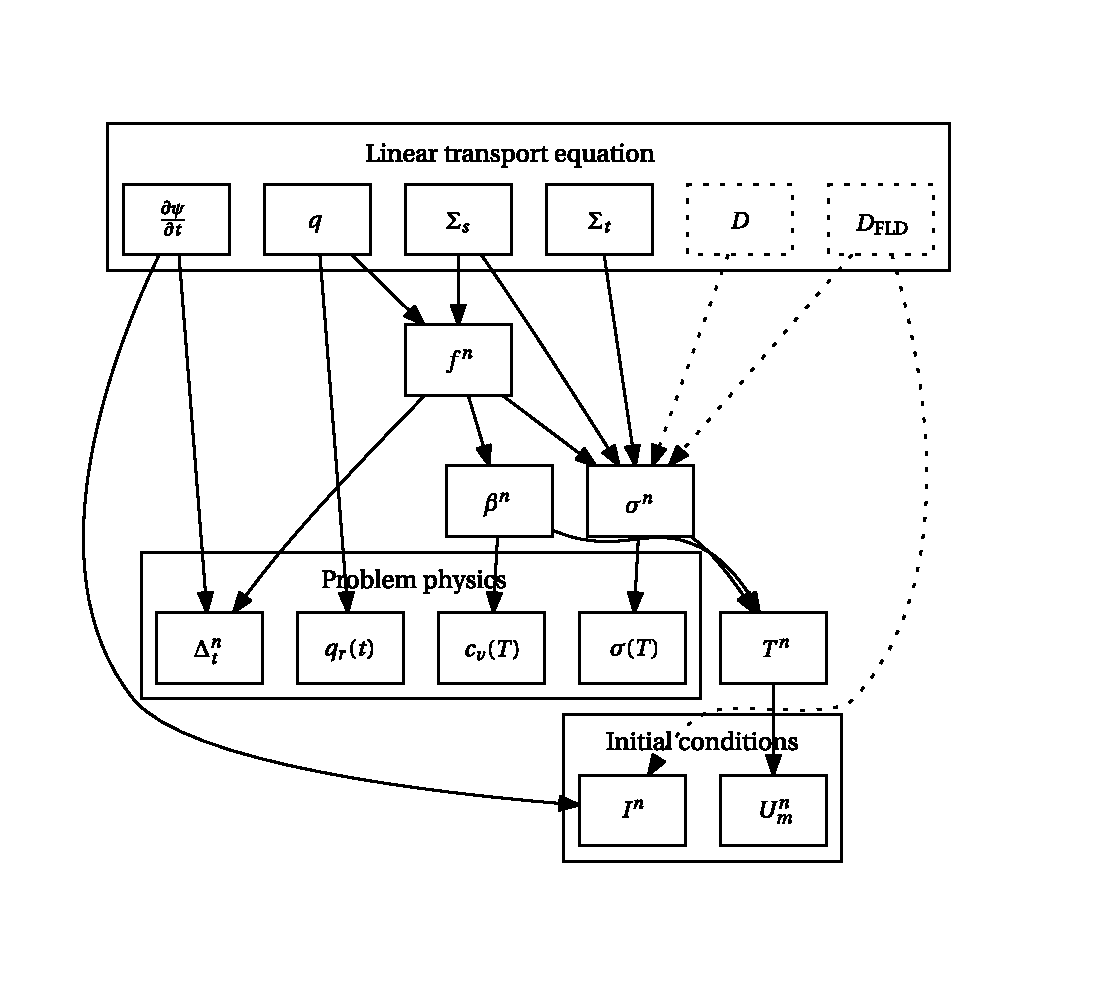
\includegraphics{semi-implicit-latex}
  \caption{Dependency graph of quantities in the semi-implicit discretization.}
  \label{fig:semiImplicitFlowchart}
\end{figure}

%%%%%%%%%%%%%%%%%%%%%%%%%%%%%%%%%%%%%%%%%%%%%%%%%%%%%%%%%%%%%%%%%%%%%%%%%%%%%%%%
\section{Deterministic radiation transport approximations}
\label{sec:bgApproxMethods}

In this section, we briefly review several existing deterministic radiation
transport methods, which discretize all unknowns in the TRT equations.

The salient difference among these methods is their treatment of
the angular dependence of the intensity. Additionally, each method tends to have
its own set of spatial discretizations that are effective and efficient for the
given angular treatment. The choice of temporal discretization is usually
independent of the method used.

Each approximation applied to the transport
equation introduces an error. The angular approximations to $I$
introduce errors that are particularly difficult to assess. Asymptotic
analysis can be used to describe quantitative regimes of applicability of most
methods \cite{Lar1983a,Ada1998a,Mor2000}, but we will confine our discussion
here to some of the qualitative
unphysical behavior introduced by the angular approximations.

Innumerable spatial discretization schemes exist. Typically, a
spatial discretization will introduce a local error into the solution with some
relation to the grid size. In the diffusion (and anisotropic diffusion) methods,
finite difference schemes are commonly used \cite{Lev2007}.

Furthermore, the treatment of the time dependence of the TRT equations is a lengthy
topic \cite{Low2004}. As in other partial differential equations, the
approximation made to the
$\tpder{I}{t}$ term (or to the time average of the other terms) incurs a
discretization error of $O(\Delta_t)$ in the case of backward Euler.
Because of the stiff nature of the TRT equations \cite{Kno2003}, unstable explicit
methods such as forward Euler are practically unusable in this application.
Furthermore, the operator split in the semi-implicit treatment produces an
$O(\Delta_t)$ linearization error. Typically, then,
higher-order methods require not only complex discretization schemes but also
iteration on the nonlinearities (or the
application of Jacobi-free Newton--Krylov techniques). In our work, we will use
only the simple semi-implicit linearization with the backward Euler implicit time
discretization. Thus, in our discussion of the methods in this section, we
represent
the transport equation in the linearized form
\begin{equation}\label{eq:siTransport}
  \frac{1}{c} \frac{I^{n+1} - I^n}{\Delta_t^n}
  + \vec{\Omega} \vd \del I^{n+1}
  + \sigma^n I^{n+1}
  = \frac{1}{4\pi} \sigma_\mathrm{es}^n \phi^{n+1}
  + \frac{1}{4\pi} Q^n\,.
\end{equation}

%%%%%%%%%%%%%%%%%%%%%%%%%%%%%%%%%%%%%%%%
\subsection{Discrete ordinates}

The discrete ordinates (\SN) method enforces the transport
equation~\eqref{eq:siTransport} only for a ``quadrature set'' of $M$ unit
directions $\vec{\Omega}_m$, giving $M$ equations
\begin{equation}\label{eq:snTransport}
  \frac{I_{m}^{n+1} - I_{m}^n}{c \Delta_t^n}
  + \vec{\Omega}_{m} \vd \del I_{m}^{n+1}
  + \sigma^n I^{n+1}
  = \frac{1}{4\pi} \sigma_\mathrm{es}^n \phi^{n+1}
  + \frac{1}{4\pi} Q^n\,,
\end{equation}
where each angle of the discrete intensity is defined as
\begin{equation*}
  I(\vec{x},\vec{\Omega}_m,t) = I_m(\vec{x},t)\,.
\end{equation*}
The equations for each ordinate are coupled at every point in space through the
scalar intensity in the scattering term:
\begin{equation*}
  \phi^{n+1} = \sum_{m=1}^M I_m^{n+1} w_m \,,
\end{equation*}
where $w_m$ is the quadrature weight corresponding to the direction
$\vec{\Omega}_m$.  The discrete equations can also be coupled at the boundaries
of a problem, e.g.~via specular reflection.

To interpret Eq.~\eqref{eq:snTransport} as a linear algebraic expression, we
rearrange it slightly:
\begin{equation*}
  \left( \vec{\Omega}_{m} \vd \del + \frac{1}{c\Delta_t^n}
  + \sigma^n \right) I_{m}^{n+1}
  = \frac{1}{c\Delta_t^n} I_{m}^n
  + \frac{1}{4\pi} \sigma_\mathrm{es}^n \phi^{n+1}
  + \frac{1}{4\pi} Q^n \,,
\end{equation*}
or, combining all $M$ equations into abstract linear operators (similar to
\cite{War2004}),
\begin{equation*}
  L \psi = S \psi + q\,.
\end{equation*}
Here $L$ is the operator representing ``streaming plus collision'' on the left
hand side, $S$ represents the isotropic redistribution of photons via
scattering, $\psi$ is the vector of unknown angular intensity at the new time
step, and $q$ is the isotropic source plus the initial condition. At every time
step, the \SN\ equations can be solved iteratively with Richardson
iteration (or ``source iteration'') \cite{Lew1984},
\begin{equation*}
  \psi^{(k+1)} = L\inv ( S \psi^{(k)} + q )\,.
\end{equation*}
Every application of $L\inv$ to the unknowns is known as a ``transport sweep,''
as it is normally implemented not as an explicit matrix of unknowns but rather in
an algorithm that sweeps across a mesh, progressively inverting the transport
equation in each cell to solve for the exiting angular intensity.
In the absence of scattering ($\sigma_\mathrm{es}^n=0$) and with specified
incident boundaries,
the \SN\ equations can be solved in only one sweep. This feature is particularly
advantageous for the anisotropic diffusion solution process.

In highly scattering systems, \SN\ can take an arbitrarily large number of
iterations to converge
using pure source iteration. Means of overcoming this---%
including diffusion
synthetic acceleration, multigrid treatments, and Krylov methods---%
exist, but these are
outside the scope of this background chapter. (Our primary use of the \SN\ method
is to calculate anisotropic diffusion coefficients.)

The grid error incurred by the spatial discretization can lead to surprisingly
inaccurate answers for optically thick, highly scattering cells
\cite{Ada1998a,Ada2001}.

%%%%%%%%%%%%%%%%%%%%%%%%%%%%%%%%%%%%%%%%
\subsection{Spherical harmonics}\label{sec:bgPn}
The spherical harmonics (\PN) method takes a very different approach to
approximating the angular dependence of the intensity. It expresses the
intensity as a truncated series of angular moments,
\begin{align*}
  I(\vec{x},\vec{\Omega},t)
  &\approx \sum_{l=0}^{L} \sum_{m=-l}^{l} Y_{l,m}(\vec{\Omega}) \left[
  \int_{4\pi} Y_{l,m}^\ast(\vec{\Omega}') I(\vec{x},\vec{\Omega}',t) \ud \Omega'
  \right]
  \\
  &= \frac{1}{4\pi} \phi(\vec{x}, t) + \frac{3}{4\pi} \vec{\Omega}\vd
  \vec{F}(\vec{x},t) + \cdots\,,
\end{align*}
where $Y_{l,m}(\vec{\Omega})$ and $Y_{l,m}^*(\vec{\Omega})$ are the spherical
harmonic functions and their complex conjugates \cite{McC2008a,Lar2007}.

The full spherical harmonic equations \cite{McC2007} are lengthy, complicated, and
largely irrelevant to our work. However, the \Pone\ equations%
\footnote{Combining the two equations yields the ``telegrapher's equation.''}%
, which result from
taking $L=1$, are indeed relevant. The first step in their derivation is to take the
zeroth and first angular moments of Eq.~\eqref{eq:siTransport}. The zeroth
angular moment of the linearized transport equation is
\begin{equation}\label{eq:p1ZerothMoment}
  \frac{\phi^{n+1} - \phi^n }{c \Delta_t}
  + \grad \vd \vec{F}
  + \sigma_\mathrm{ea}^n \phi^{n+1}
  = Q^n\,,
\end{equation}
and the first moment is the vector equation
\begin{equation}\label{eq:p1FirstMoment}
  \frac{\vec{F}^{n+1} - \vec{F}^n }{c \Delta_t} + \grad \vd \int_{4\pi}
  \vec{\Omega}\vec{\Omega} I^{n+1} \ud\Omega
  + \sigma^n \vec{F}^{n+1}
  = 0\,.
\end{equation}

The \Pone\ approximation provides a closure for Eq.~\eqref{eq:p1FirstMoment} by
approximating the intensity as
\begin{equation}\label{eq:p1Approx}
  I^{n+1}(\vec{x},\vec{\Omega})
  \approx \frac{1}{4\pi} \phi^{n+1}(\vec{x})
  + \frac{3}{4\pi} \vec{\Omega}\vd \vec{F}^{n+1}(\vec{x}) \,.
\end{equation}
Thus, the second angular moment is
\begin{equation*}
  \int_{4\pi} \vec{\Omega}\vec{\Omega} I^{n+1} \ud\Omega
  \approx \frac{1}{4\pi} \phi^{n+1}
  \int_{4\pi} \vec{\Omega}\vec{\Omega}\ud\Omega + 0
  = \frac{1}{3} \Identitytens \phi^{n+1}\,,
\end{equation*}
where $\Identitytens$ is the identity matrix (the unit dyad).
Equation~\eqref{eq:p1FirstMoment} becomes
\begin{equation} \label{eq:p1FirstMoment2}
  \frac{\vec{F}^{n+1} - \vec{F}^n }{c \Delta_t} + \frac{1}{3} \grad \phi^{n+1}
  + \sigma^n \vec{F}^{n+1}
  = 0\,.
\end{equation}

Rather than the $M$ unknowns per spatial coordinate of the \SN\ method, the
\Pone\ has four (or, in 2-D space, three). It is therefore easier to solve and
store in computer memory. Unfortunately, the disadvantages of \Pone\ are
pronounced..
First, most obviously, the linear-in-angle approximation is not generally valid, so
the solution will
usually lag in accuracy compared to a transport method. Second, it happens that
the approximation in Eq.~\eqref{eq:p1FirstMoment2} yields a plane wave
propagation speed of $c/\sqrt{3}$ rather than the physical $c$
\cite{Mih1984,War2002}. Even worse, the \Pone\ equation and in fact the entire
\PN\ family can produce negative solutions for $\phi^{n+1}$ in the presence of
steep gradients \cite{Bru2002,McC2007,McC2008a}. This is a significant problem
in TRT
applications because a negative $\phi$ can lead to a negative material
temperature and
the catastrophic failure of a simulation.

An alternative to using the linear-in-angle approximation in the closure for the
second angular moment
$\int_{4\pi} \vec{\Omega}\vec{\Omega} I^{n+1} \ud\Omega$ is to define an
Eddington tensor \cite{Pom1982,Ols2000} as
\begin{equation*}
  \Etens \equiv \frac{\int_{4\pi} \vec{\Omega}\vec{\Omega} I^{n+1}
  \ud\Omega}{\int_{4\pi} I^{n+1} \ud\Omega}\,,
\end{equation*}
so that Eq.~\eqref{eq:p1FirstMoment} becomes
\begin{equation*}
  \frac{\vec{F}^{n+1} - \vec{F}^n }{c \Delta_t}
  + \grad \vd \left( \Etens\phi^{n+1} \right)
  + \sigma^n \vec{F}^{n+1}
  = 0\,.
\end{equation*}
Typically, $\Etens$ is calculated via a transport problem or some \emph{a
priori} estimated relationship between $\phi$ and its gradient.
The variable Eddington factor, or quasidiffusion, family of methods can be much
more accurate than the \Pone\ equations, but the nonlinear closure for $\Etens$
can lead to nonphysical shocks and numerical instabilities \cite{Ols2000}.

%%%%%%%%%%%%%%%%%%%%%%%%%%%%%%%%%%%%%%%%
\subsection{Diffusion}\label{sec:bgDiffusion}

After the \Pone\ approximation is applied to the first angular moment of the
transport equation, Eq.~\eqref{eq:p1Approx}, one further simplification leads to
the very common diffusion approximation. The ``quasi-static'' \cite{Dud1976}
approximation is to discard the time derivative term in the first angular moment,
Eq.~\eqref{eq:p1FirstMoment}, simplifying the expression and allowing for an
explicit solution of $\vec{F}^{n+1}$ to yield Fick's law:
\begin{equation*}
  \vec{F}^{n+1} = - \frac{1}{3\sigma^n} \grad \phi^{n+1}\,.
\end{equation*}
This simple expression approximates the entire angular distribution of the
intensity $I$ using a single unknown, yielding a very small memory footprint and
a typically very fast solution.

However, Fick's law is only a coarse approximation, and it is not
necessarily accurate. An asymptotic analysis \cite{Lar1975,Lar1983a} shows that
the diffusion approximation indeed is a leading
order solution of the transport equation given certain conditions---%
primarily, that the material properties vary slowly in space, and that the
system is highly scattering. However, for problems that have a fast time scale
or contain strongly absorbing materials, the diffusion approximation will not
yield transport-quality answers.

Furthermore, the time-dependent diffusion approximation yields a parabolic equation
for $\phi$, allowing energy to be transferred faster than the speed of light. This
often severe shortcoming is addressed in a method known as \emph{flux-limited
diffusion}, which is discussed next.

%%%%%%%%%%%%%%%%%%%%%%%%%%%%%%%%%%%%%%%%
\subsection{Flux-limited diffusion}\label{sec:bgFld}

The exact radiation intensity satisfies the mathematical identity $\norm{F} \le
\phi$,
essentially limiting the leakage of radiation at a point to the radiation
energy at that point. The identity can be shown using the triangle inequality:
\begin{align}
  \norm{\vec{F}} &= \norm{ \int_{4\pi} \vec{\Omega} I \ud \Omega}
  \\ \nonumber
  &\le \int_{4\pi} \norm{\vec{\Omega}} \abs{I} \ud \Omega 
  \\ \nonumber
  &\le \int_{4\pi} [1] I \ud\Omega
  \\ \label{eq:fluxLimit}
  \norm{\vec{F}} &\le \phi\,.
  \\ 
  \intertext{Substituting Fick's law for $\vec{F}$ gives a condition that
  shows when the
  diffusion coefficient satisfies this limit:} \nonumber
  \norm{- D \grad \phi} &\le \phi
  \\ \label{eq:fluxLimitDiffusion}
  \norm{\grad \phi} & \le \frac{\phi}{D} \,.
\end{align}
In an optically thin region, $\sigma\approx 0$, $D\to\infty$, and this condition
will usually be violated. Additionally, the large radiation energy gradient at a
wavefront can lead to a violation of the limit.

A \emph{flux limiter} is designed to combat these problems by enforcing
Eq.~\eqref{eq:fluxLimitDiffusion} through an \emph{ad hoc} modification to
the definition of $D$.
Although certain flux limiters \cite{Lev1984} are based on
idealized models that the radiation intensity might take in an optically thin
region, the usual approach is more
straightforward. The flux-limited diffusion (FLD) coefficient should approach the
standard diffusion coefficient $1/3\sigma$ when the spatial gradients are weak,
but it should satisfy Eq.~\eqref{eq:fluxLimit} when the gradients are strong.
A standard formulation \cite{Ols2000} is
\begin{equation} \label{eq:fluxLimiter}
  D = \left[ (3\sigma)^{m} + \left( \frac{\norm{\grad
  \phi}}{\phi} \right)^{m}\right]^{-1/m} \,.
\end{equation}
The ``sum'' limiter at $m=1$ due to Wilson \cite{Mor2000} leads to inaccuracies
at the diffusion limit, but using the ``square-root'' limiter at $m=2$ (as
suggested by Larsen \cite{Ols2000}) is accurate to leading order. Taking
$m\to\infty$ leads to the ``max'' limiter,
\begin{equation} \label{eq:fluxLimiterMax}
  D = \max\left( 3\sigma, \frac{\norm{\grad \phi}}{\phi}
  \right)\inv\,,
\end{equation}
which is also accurate in the
diffusion limit but has discontinuous derivatives.

Typically, Eq.~\eqref{eq:fluxLimiter} is evaluated explicitly or ``lagged''
because of its inherent nonlinearity, giving the following FLD version of Fick's
law:
\begin{equation*}
  \vec{F}^{n+1} \approx - \left[ (3\sigma)^{m} + \left( \frac{\norm{\grad
  \phi^{n}}}{\phi^{n}} \right)^{m}\right]^{-1/m} \grad \phi^{n+1} \,.
\end{equation*}

The discretization of the normalized gradient in Eq.~\eqref{eq:fluxLimiter}
adds an extra minor complication to FLD. The implementation
used in this thesis takes a geometric average of the normalized gradient on the
face of a computational cell as suggested by \cite{Ols2007}:
\begin{multline*}
 \frac{1}{\phi} \frac{\partial \phi}{\partial x}
  \approx
\sqrt{\abs{ \left(  \frac{1}{(\phi_{i+1} + \phi_{i})/2} \frac{\phi_{i+1} - \phi_{i}}
 { (\Delta_{x,i+1}/2 + \Delta_{x,i}/2)} \right)
\left(  \frac{1}{(\phi_{i} + \phi_{i-1})/2} \frac{\phi_{i} - \phi_{i-1}}
{ (\Delta_{x,i}/2 + \Delta_{x,i-1}/2)} \right) }}
\\
\times
 \mathrm{sgn}(\phi_{i+1} - \phi_{i-1})\,,
\end{multline*}
rather than the arithmetic average
\begin{equation*}
 \frac{1}{\phi} \frac{\partial \phi}{\partial x}
  \approx
 \frac{1}{\phi_{i}} \frac{\phi_{i+1} - \phi_{i-1}}
 { (\Delta_{x,i+1}/2 + \Delta_{x,i} + \Delta_{x,i-1}/2)}\,.
\end{equation*}

%%%%%%%%%%%%%%%%%%%%%%%%%%%%%%%%%%%%%%%%%%%%%%%%%%%%%%%%%%%%%%%%%%%%%%%%%%%%%%%%
\section{Summary}

This chapter provides an overview of the equations underlying thermal
radiative transfer, as well as some existing techniques for solving these
equations. We have discussed some of the strengths and weaknesses of several
deterministic methods that will compete with the new anisotropic diffusion
approximation method, which is discussed next.

